% Group 7 - IEEE report, Data Labelling section only (Prabhav Pradeep, CH24BTECH11029)
% Uses the course IEEE template (ieee_conference_4page_template.tex).
% Teammates: copy everything between "BEGIN DATA LABELLING" and "END DATA LABELLING"
% into the group report, and copy the figures/ folder next to the group .tex.
% Needs only amsmath/amssymb, graphicx and booktabs, already in the template.
% Compile with: pdflatex data_labelling_section.tex

\documentclass[conference]{IEEEtran}

% -------------------- Packages --------------------
\usepackage{cite}
\usepackage{amsmath,amssymb,amsfonts}
\usepackage{graphicx}
\usepackage{booktabs}
\usepackage{multirow}
\usepackage{url}
\usepackage{array}
\usepackage{xcolor}
\usepackage{siunitx}
\usepackage[T1]{fontenc}

% -------------------- Paper information --------------------
\title{Stress-Granule Detection: Data Labelling}

\author{\IEEEauthorblockN{Group 7 --- Prabhav Pradeep (CH24BTECH11029)}}

\begin{document}
\maketitle

% ======================= BEGIN DATA LABELLING =======================
\section{Data Labelling}
\label{sec:labelling}

\textbf{Strategy.} Training labels are produced \emph{automatically} by a
classical labeller on videos 1 and 2 (105 frames). The final (V4) dataset
has 1{,}487 tiles of $256\times256$\,px and 13{,}507 granules. Each tile has
a granule mask, granule and cell instance images, and YOLO boxes. The tiles
are split into 5 folds grouped by grid position, so the same cells never
appear in both training and test data. Video 3 is never used for training.
From it, 19 tiles (5 frames, 7 positions) were uploaded to Roboflow, and 8
of them (102 granules) were outlined \emph{manually} with polygons
(Fig.~\ref{fig:hand}). These hand labels are the fixed answer key for every
label version and every network. A prediction is a true positive (TP) if
its IoU with a hand granule is at least 0.5; \emph{capture} is the share of
hand granules of which at least half the pixels are predicted.

\begin{figure}[!t]
    \centering
    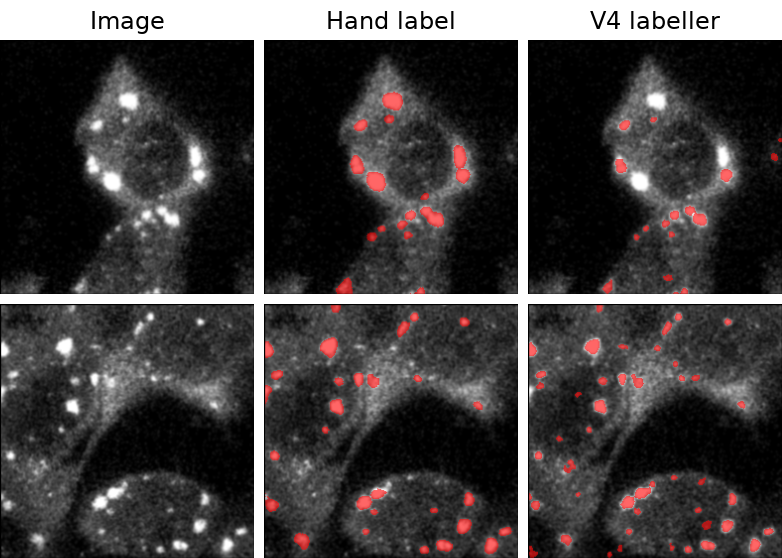
\includegraphics[width=0.62\linewidth]{figures/hand_vs_auto}
    \caption{Held-out video-3 tiles: manual and automatic (V4) labels
    (red = granule).}
    \label{fig:hand}
\end{figure}

\textbf{Cell mask.} Each pixel is described by
$\mathbf{x}=(\sqrt{I},\log(1+D))$, where $I\in[0,1]$ is the intensity and
$D$ the optical-flow magnitude. A three-component Gaussian mixture is fitted
to $2\times10^5$ sampled pixels. The two darkest components are background;
the third is cell:
\begin{equation}
P(\text{cell}\mid\mathbf{x})=\frac{\pi_c\,\mathcal{N}(\mathbf{x};\boldsymbol{\mu}_c,\boldsymbol{\Sigma}_c)}
{\sum_{j=1}^{3}\pi_j\,\mathcal{N}(\mathbf{x};\boldsymbol{\mu}_j,\boldsymbol{\Sigma}_j)}
\cdot\frac{1}{1+e^{-(I-I_0)/0.005}} .
\label{eq:gmm}
\end{equation}
The sigmoid gate stops motion alone from making a dark pixel a cell pixel.
$I_0$ is the lowest intensity at which a still pixel ($D=0$) has $P>0.5$.

\textbf{Top-hat contrast.} Cell brightness varies about $10\times$, so a
global threshold fails. With $I_s=G_1*I$ and pixels outside cells filled by
normalised convolution, the background is the smoothed grey-scale opening
with a disk $B_r$:
\begin{equation}
b=G_{r/2}*(I_s\circ B_r),\qquad S=\frac{I_s-b}{b+0.05}.
\label{eq:tophat}
\end{equation}
The opening $(I\ominus B_r)\oplus B_r$ removes every bright structure that
$B_r$ does not fit inside. The top-hat $I_s-b$ therefore keeps only the
puncta, and dividing by $b$ makes it a relative contrast, comparable across
bright and dim cells. A granule wider than $B_r$ is absorbed into $b$, so
$r$ must exceed the largest granule radius.

\textbf{Hessian blobs.} From
$I(\mathbf{p}+\mathbf{h})\approx I+\nabla I^{\top}\mathbf{h}+\tfrac12\mathbf{h}^{\top}\mathbf{H}\mathbf{h}$,
both eigenvalues $\lambda_1\ge\lambda_2$ of $\mathbf{H}$ are strongly
negative at a bright blob, while $\lambda_1\approx0$ on a ridge such as a
cell rim. The blob response is
\begin{equation}
\mathcal{B}=\max_{\sigma}\,\sigma^{2}\max(0,-\lambda_1(\sigma)),
\label{eq:blob}
\end{equation}
where $\sigma^2$ normalises the second derivatives across scales, so the
response peaks at blob radius $\approx1.4\sigma$.

\textbf{Seeds and growth.} Seeds are local maxima inside cells where
\begin{equation}
\frac{\mathcal{B}}{b+0.05}>\operatorname{med}+k\cdot1.4826\cdot\operatorname{MAD},\qquad S\ge S_{\min}.
\label{eq:mad}
\end{equation}
The factor 1.4826 makes the MAD a consistent estimate of $\sigma_{\text{noise}}$,
and its 50\% breakdown point stops the granules from raising their own
threshold. Each seed $p$ is grown by a watershed down to half its peak
height, $b_p+0.5(I_p-b_p)$, within $\min(R,\,2.5\sigma_p+2)$\,px of the
seed. A region is kept if its area is within the version's limits,
eccentricity $\le0.95$, solidity $\ge0.7$, and it is not on a saturated
blob. Label caches are named after their settings, so new settings cannot
silently reload old labels. Re-running the code with V1 settings gives 362
granules on a test frame, against 366 stored.

\begin{figure*}[!t]
    \centering
    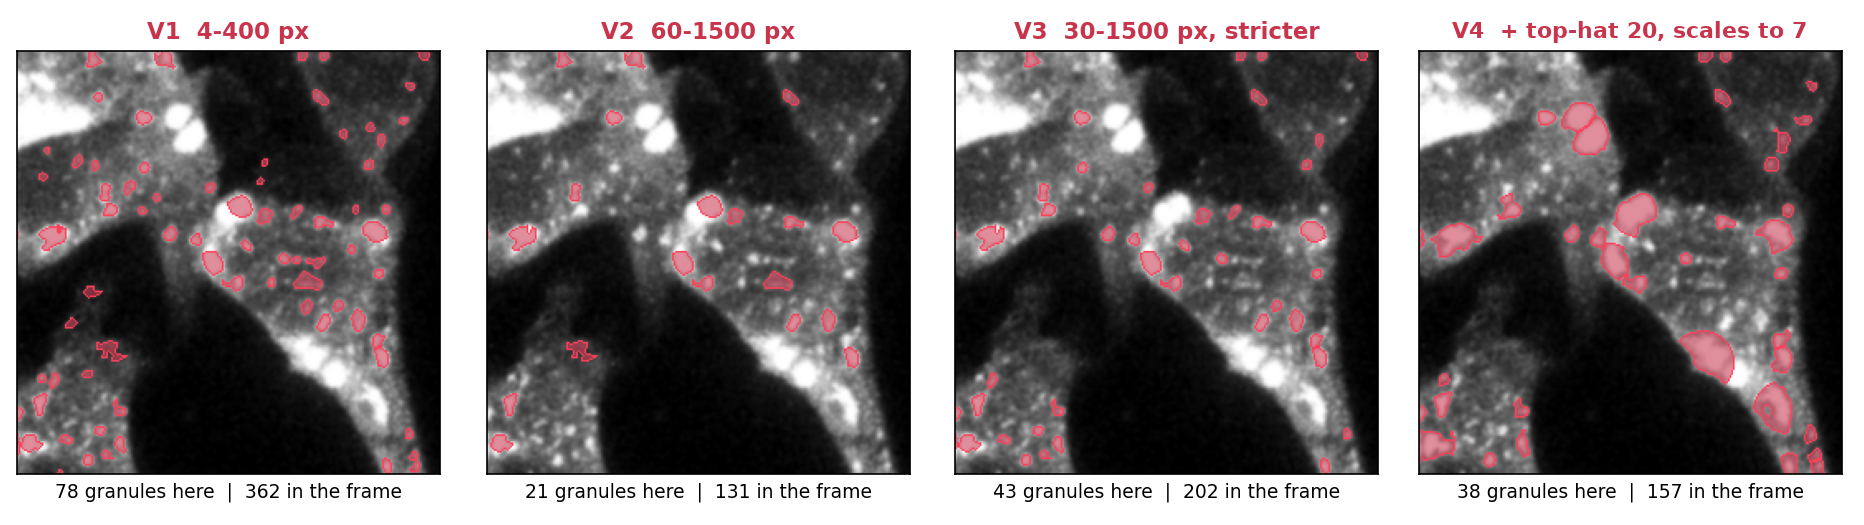
\includegraphics[width=0.78\textwidth]{figures/label_versions_strip}
    \caption{Output of each labeller version on the same region (video 1,
    frame 10), with granule counts for this crop and for the whole frame.}
    \label{fig:versions}
\end{figure*}

\begin{table}[!t]
    \centering
    \caption{Label versions (granules: videos 1+2) and U-Net trained on
    each, scored on the 8 hand-labelled tiles (mean of 5 checkpoints).}
    \label{tab:versions}
    \footnotesize
    \setlength{\tabcolsep}{2.2pt}
    \begin{tabular}{@{}llrccccr@{}}
        \toprule
        & Change & Gran. & P & R & F1 & Dice & FP \\
        \midrule
        V1 & area 4--400\,px                        & 22{,}283 & 0.23 & 0.73 & 0.34 & 0.53 & $\sim$250 \\
        V2 & area 60--1500, $R$ 12$\to$22            &  7{,}998 & 0.49 & 0.38 & 0.37 & 0.52 & 41 \\
        V3 & 30--1500, $k$=5, $S_{\min}$=0.7         & 13{,}039 & 0.43 & 0.66 & 0.46 & 0.55 & 88 \\
        V4 & $r$ 8$\to$20, $\sigma_{\max}$ 3.5$\to$7  & 13{,}507 & 0.49 & 0.71 & 0.52 & 0.70 & 75 \\
        \multicolumn{2}{@{}l}{V4 + blob filter ($<$20\,px)} & & \textbf{0.56} & \textbf{0.71} & \textbf{0.57} & \textbf{0.71} & \textbf{56} \\
        \bottomrule
    \end{tabular}
\end{table}

\textbf{Label versions.} The labeller went through four versions
(Table~\ref{tab:versions}, Fig.~\ref{fig:versions}). After each one all
networks were retrained and scored on the same hand tiles.
\emph{V1} counted every 4--400\,px spot, so U-Net found most granules
(recall 0.73) but 3 of every 4 detections were wrong.
\emph{V2} dropped blobs under 60\,px, as feedback asked for fewer false
positives. Precision doubled, but real 30--60\,px granules were lost
(recall 0.38).
\emph{V3} restored the 30\,px minimum with a stricter brightness test
(recall 0.66).
\emph{V4} widened the top-hat ($r=20$\,px) and the blob scales
($\sigma\le7$). Before, granules wider than about 14\,px were hollowed out
or missed; now they are outlined in full. Dice rose from 0.55 to 0.70, and
V4 recovers V1's recall at twice its precision.

Every network gains from V2 to V4 (F1 on the hand tiles): NoSkip
0.36$\to$0.48, U-Net 0.37$\to$0.52, AttU-Net 0.35$\to$0.54, DWU-Net
0.35$\to$0.51, DWAttU-Net 0.36$\to$0.51. The gain comes from the labels, not
from one architecture. Scored directly, the labeller itself improves from
F1 0.38 (V1; 130 FP) to 0.53 (V4; P 0.58, R 0.64, 40 FP, 7 tiles), while a
DoG detector reaches 0.22 (recall 0.79 but 714 FP). On the same tiles the
networks reach 0.48--0.52, about as good as the labeller they learned from.
Against each version's \emph{own} labels, 5-fold U-Net F1 is 0.71, 0.62,
0.69 and 0.66 for V1--V4. This measures how well a network copies its
labeller, not label quality: V1 scores highest yet is worst on the hand
tiles.

\textbf{Errors by size.} Large granules are found reliably. For hand
granules of at least 150\,px (31 granules), U-Net recall is 0.80 and capture
99\%; for 30--150\,px, recall is 0.68 and capture 77\%. The V1 labeller
found none of the 4 granules over 400\,px. False positives are mostly tiny:
44\% of U-Net's (33 of 75) are under 30\,px, a size the labels never contain.
On the 5-fold sets, granules of at least 150\,px have recall 0.64, and about
a fifth of them are merged with a neighbour. A \emph{blob filter} deletes
predicted blobs under $N$\,px, with no retraining. $N$ was chosen on
validation tiles only, where every network peaks at $N=20$. On the hand
tiles, precision rises from 0.49 to 0.56 at unchanged recall 0.71, and false
positives fall from 75 to 56. On the 5-fold test sets, precision rises from
0.64 to 0.72 and F1 from 0.66 to 0.70. At $N=40$, hand-tile recall falls to
0.57.

\textbf{Perimeter and time.} Hand-labelled granules have a median perimeter
of 35\,px, and 64\% lie between 20 and 45\,px. U-Net outlines are within 7\%
of the labeller's but 14\% shorter than hand-drawn ones. In video 1
(0--60\,min), labelled granules per tile rise from 6.2 to 13.3 while their
mean perimeter falls from 62 to 34\,px ($p<0.001$, Pearson test on a linear
fit), so many small new granules form. In video 2 (60--120\,min) both
change only slightly. U-Net follows the same trends but over-counts.
% ======================== END DATA LABELLING ========================

\end{document}
